% arara: pdflatex
% !arara: indent: {overwrite: yes}
\documentclass{article}
\usepackage[margin=0.5cm,bottom=2cm]{geometry}
\usepackage{kpfonts}
\usepackage{eso-pic}                % put things into background 
\usepackage{transparent}
\usepackage{tcolorbox}

\tcbuselibrary{skins}


\AddToShipoutPicture{% from package eso-pic: put something to the background
	\AtPageCenter{% start the bar at the bottom right of the page
		\put(-\LenToUnit{.45\paperwidth},-\LenToUnit{.4\paperheight}){% move it to the middle
			%{\transparent{.4}{\includegraphics[width=20cm]{pcclogo}}}
			{\transparent{.5}{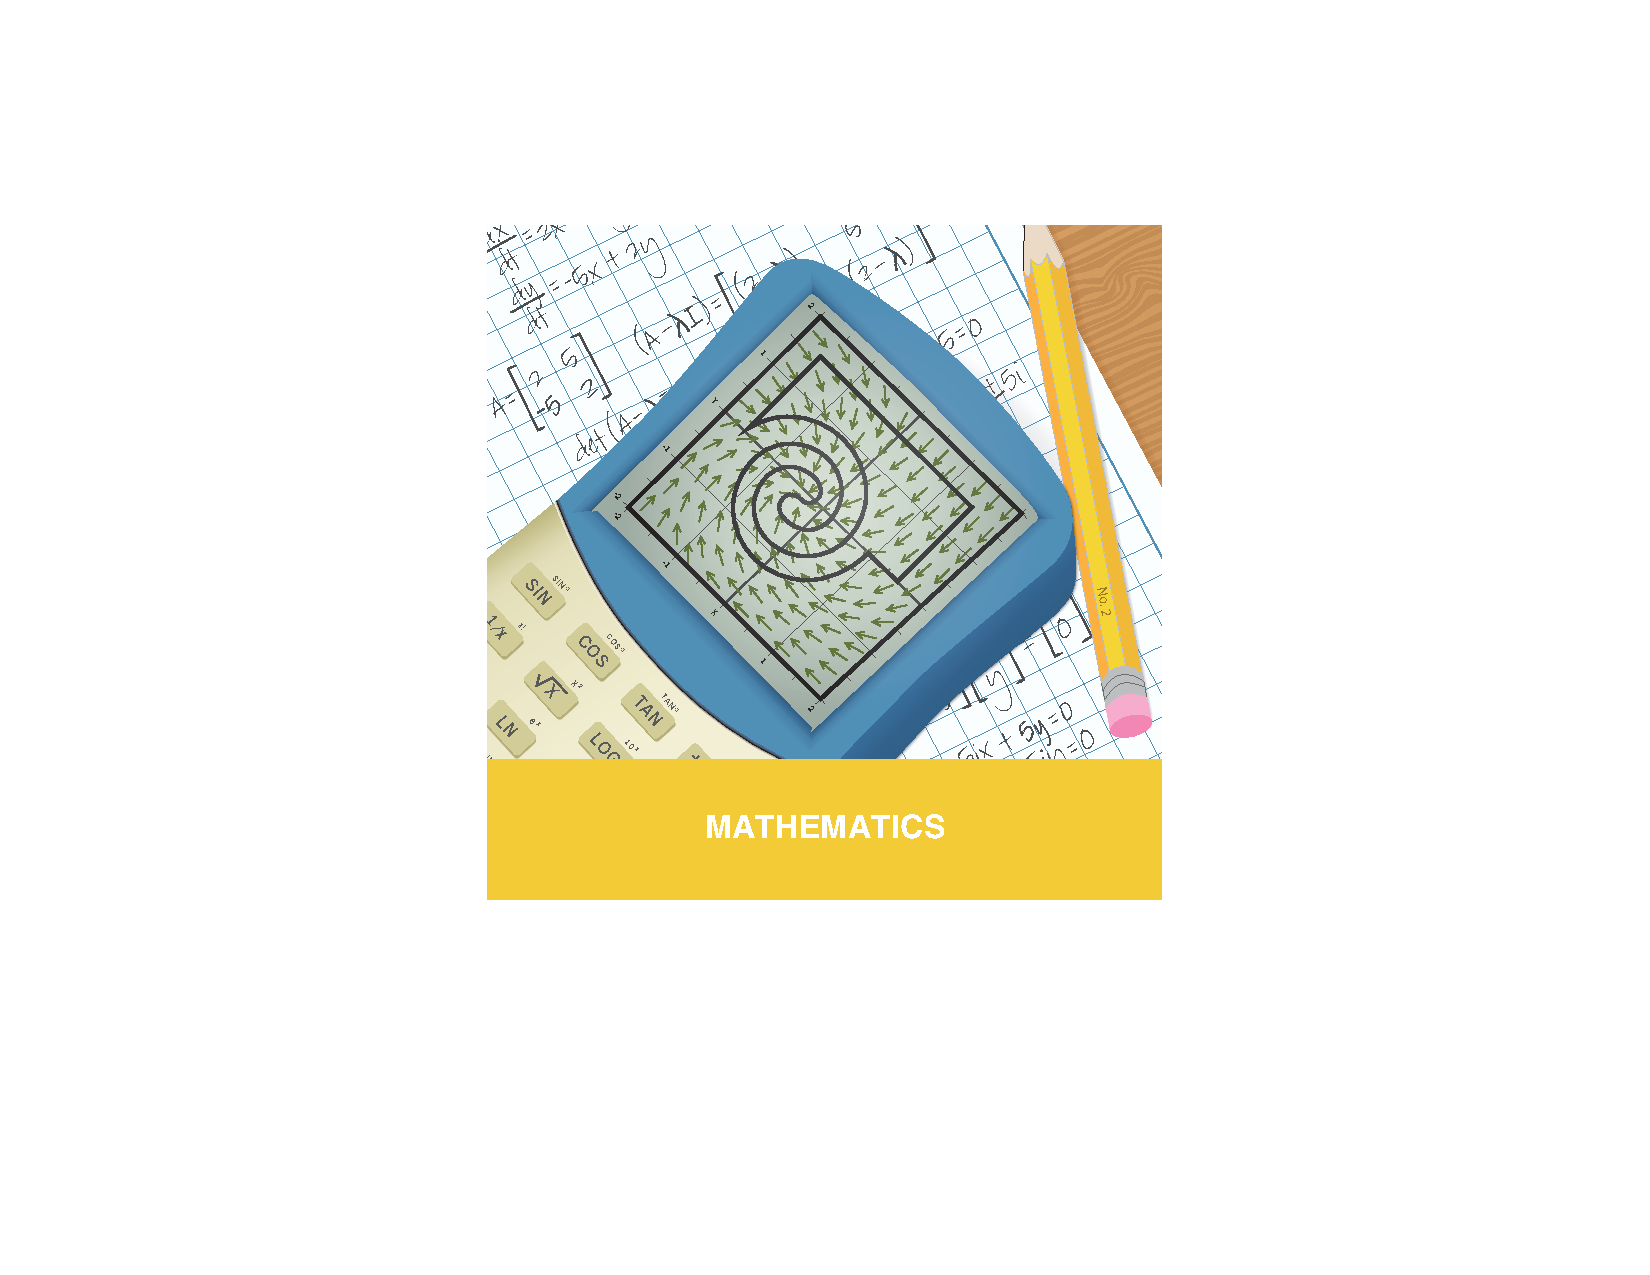
\includegraphics[width=20cm]{50th_mathematicsproof}}}
		}%
	}%
	\AtPageLowerLeft{% start the bar at the bottom right of the page
		\put(\LenToUnit{\dimexpr\paperwidth-3cm},0){% move it to the top right
			\color{blue}\rule{3cm}{\LenToUnit\paperheight}%
		}%
	}%
}

\pagestyle{empty}
\newsavebox\mybox
\begin{document}

\global\sbox{\mybox}{%
	\begin{tcolorbox}[enhanced,flushright upper,
			width=6.8cm,boxrule=0.4pt,
			colback=white,colframe=black!50!yellow,
		drop fuzzy midday shadow=black!50!yellow]
		{\bfseries\LARGE {Program Review} \par}
		{\large \itshape Mathematics \par}
		{\large Portland Community College }
	\end{tcolorbox}
}

\vspace*{1cm}
\mbox{}\hfill\scalebox{2}{\usebox{\mybox}}

%\mbox{}\hfill\scalebox{-1}{\usebox{\mybox}}
%\rotatebox{180}{\usebox{\mybox}}

\vfill

\centering
\vspace*{1cm}

%    \huge Fall 2008--Spring 2013
\global\sbox{\mybox}{%
	\begin{tcolorbox}[enhanced,
			width=4.8cm,boxrule=1.4pt,
			colback=white,colframe=black!50!yellow,
		]
		{\scshape Fall 2008--Spring 2013}
	\end{tcolorbox}
}

\mbox{}\scalebox{2}{\usebox{\mybox}}\mbox{}\hfill
\end{document}
